\section{Electrical Specifications}

This section details the electrical characteristics, operating conditions, and timing requirements for the Micro-CUDA cluster hardware.

\subsection{Absolute Maximum Ratings}
Stresses beyond those listed in Table \ref{tab:abs_ratings} may cause permanent damage to the device.

\begin{table}[h]
\centering
\caption{Absolute Maximum Ratings}
\label{tab:abs_ratings}
\resizebox{0.95\columnwidth}{!}{%
\begin{tabular}{|l|l|c|c|c|}
\hline
\textbf{Symbol} & \textbf{Parameter} & \textbf{Min} & \textbf{Max} & \textbf{Unit} \\ \hline
$V_{CC}$ & Supply Voltage (VSYS) & -0.3 & 5.5 & V \\ \hline
$V_{IO}$ & GPIO Input Voltage & -0.3 & $V_{CC} + 0.3$ & V \\ \hline
$I_{total}$ & Total Current Source/Sink & - & 1200 & mA \\ \hline
$T_{str}$ & Storage Temperature & -40 & 125 & $^{\circ}$C \\ \hline
\end{tabular}%
}
\end{table}

\subsection{Characteristics}
Operating conditions: $V_{CC} = 5.0V$, $T_{A} = 25^{\circ}C$ unless otherwise noted.

\begin{table}[h]
\centering
\caption{DC Electrical Characteristics}
\label{tab:dc_chars}
\resizebox{0.95\columnwidth}{!}{%
\begin{tabular}{|l|l|l|c|c|c|}
\hline
\textbf{Symbol} & \textbf{Parameter} & \textbf{Condition} & \textbf{Min} & \textbf{Max} & \textbf{Unit} \\ \hline
$V_{IH}$ & Input High Voltage & - & 2.0 & $V_{CC}$ & V \\ \hline
$V_{IL}$ & Input Low Voltage & - & -0.3 & 0.8 & V \\ \hline
$V_{OH}$ & Output High Voltage & $I_{OH} = -12mA$ & 2.4 & - & V \\ \hline
$V_{OL}$ & Output Low Voltage & $I_{OL} = 12mA$ & - & 0.4 & V \\ \hline
$I_{idle}$ & Idle Current & No computation & - & 80 & mA \\ \hline
$I_{load}$ & Full Load Current & All Cores Active & - & 950 & mA \\ \hline
\end{tabular}%
}
\end{table}

\subsection{AC Timing Analysis}
The Global G-BUS operates at 50MHz. Figure \ref{fig:ac_timing} illustrates the timing budget required to ensure signal integrity across the split-bus topology.

\begin{figure}[htbp]
\centering
\resizebox{0.95\columnwidth}{!}{%
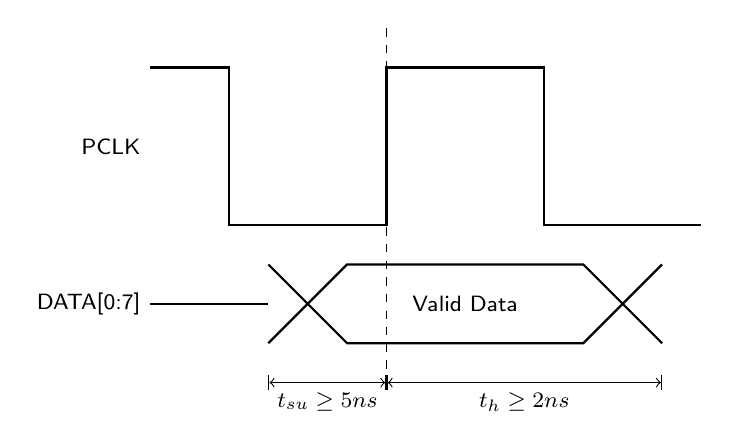
\begin{tikzpicture}[
    font=\sffamily\footnotesize,
    timing/.style={thick}
]
    % Clock
    \draw[timing] (0, 2) -- (1, 2) -- (1, 0) -- (3, 0) -- (3, 2) -- (5, 2) -- (5, 0) -- (7, 0);
    \node[left] at (0, 1) {PCLK};
    
    % Data
    \draw[timing] (0, -1) -- (1.5, -1);
    \draw[timing] (1.5, -1.5) -- (2.5, -0.5) -- (5.5, -0.5) -- (6.5, -1.5);
    \draw[timing] (1.5, -0.5) -- (2.5, -1.5) -- (5.5, -1.5) -- (6.5, -0.5);
    \node[left] at (0, -1) {DATA[0:7]};
    
    % Valid Window
    \draw[dashed] (3, 2.5) -- (3, -2); % Clock Edge
    
    % Dimensions
    \draw[|<->|] (1.5, -2) -- (3, -2) node[midway, below] {$t_{su} \ge 5ns$};
    \draw[|<->|] (3, -2) -- (6.5, -2) node[midway, below] {$t_{h} \ge 2ns$};
    
    \node at (4, -1) {Valid Data};
\end{tikzpicture}
}
\caption{AC Timing Diagram for Global G-BUS. The setup time ($t_{su}$) allows for propagation delay across the 10cm bus trace.}
\label{fig:ac_timing}
\end{figure}
